\documentclass[border=3pt]{standalone}
% Preâmbulo compartilhado pelos diagramas TikZ da aula 7 (Filtros Não Paramétricos)
\usepackage[T1]{fontenc}
\usepackage[utf8]{inputenc}
\usepackage{lmodern}
\usepackage{amsmath}
\usepackage{xcolor}
\usepackage{tikz}
\usetikzlibrary{arrows.meta,angles,quotes,decorations.pathmorphing,calc,
                positioning,shapes.geometric,shapes.misc,backgrounds,fit,
                math}

% Paleta (mesma dos SVGs originais)
\definecolor{dblue}{HTML}{2A5B8C}
\definecolor{dorange}{HTML}{B3541E}
\definecolor{dgreen}{HTML}{4A7C59}
\definecolor{dred}{HTML}{9C4B4B}
\definecolor{dcream}{HTML}{F4F1EA}
\definecolor{dshade}{HTML}{DDD7C9}

% Função gaussiana (não normalizada por padrão de escala visual)
\pgfmathdeclarefunction{gauss}{3}{%
  \pgfmathparse{1/(#3*sqrt(2*pi))*exp(-((#1-#2)^2)/(2*#3^2))}%
}

% Estilos comuns (prefixo d... para não colidir com chaves internas do pgf)
\tikzset{
  >={Stealth[length=2mm]},
  dguide/.style={gray!55, dashed, line width=0.4pt},
  daxis/.style={gray!60, line width=0.7pt, ->},
  dbody/.style={fill=black!3, draw=black!80, line width=1pt},
  dacc/.style={draw=dblue, line width=1pt},
  dlbl/.style={black!55, font=\small},
  dsub/.style={black!45, font=\footnotesize},
  dstate/.style={circle, draw=black!80, fill=dcream, line width=1pt,
                 minimum size=17mm, font=\large, inner sep=1pt},
  dobs/.style={circle, draw=black!80, fill=dshade, line width=1pt,
               minimum size=14mm, font=\large, inner sep=1pt},
  dbox/.style={rounded corners=2pt, draw=black!80, fill=dcream, line width=1pt,
               align=center, inner sep=6pt},
  dop/.style={circle, draw=black!80, fill=white, line width=1pt,
              minimum size=6mm, inner sep=0pt, font=\small},
  dtrans/.style={->, dblue, line width=1pt},
  dmeas/.style={->, dorange, line width=1pt},
  dcurve/.style={line width=1pt, dblue},
  dcurveb/.style={line width=1.4pt, dorange},
}

\begin{document}
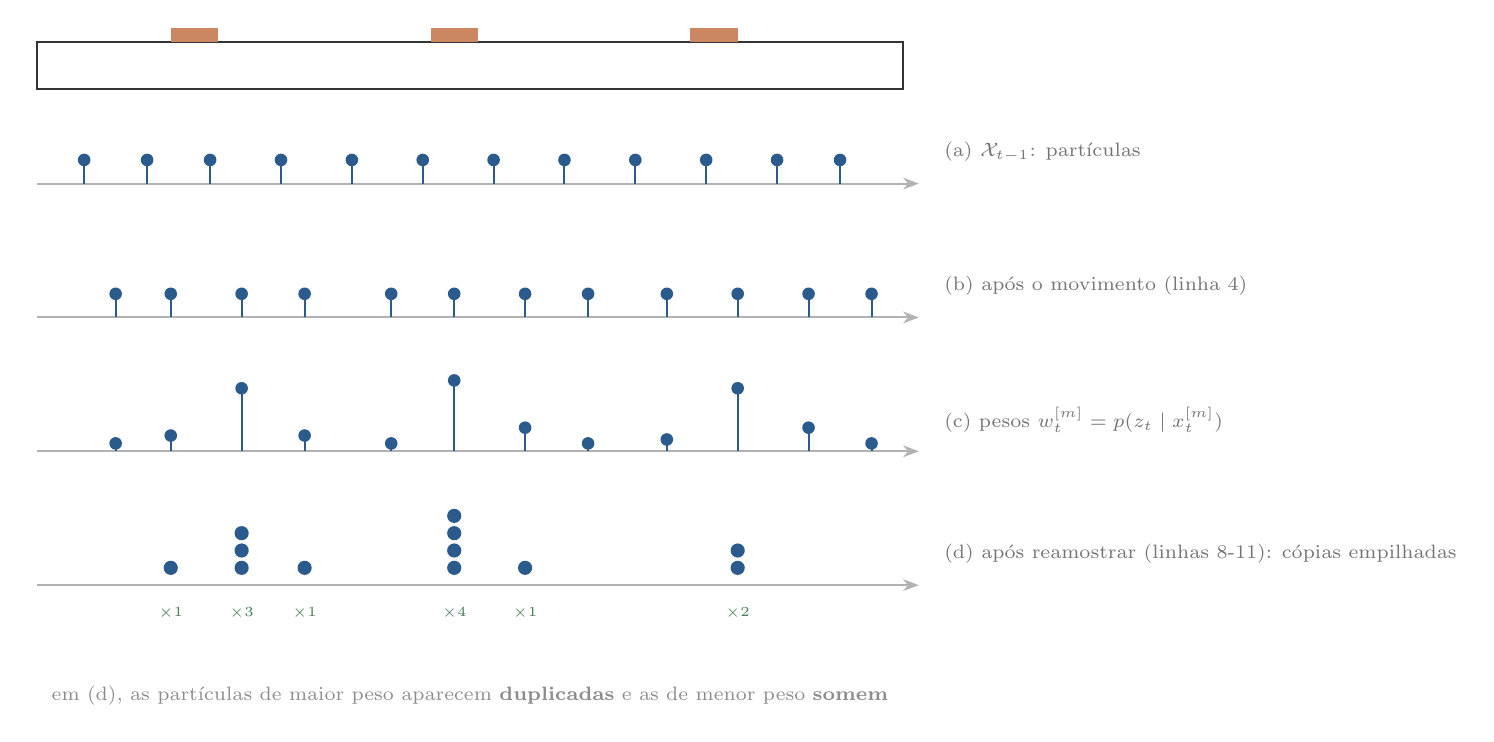
\begin{tikzpicture}[x=1cm,y=1cm]
  \draw[dbody, fill=white, line width=0.9pt] (0,8.2) rectangle (11,8.8); \foreach \d in {2.0,5.3,8.6} { \fill[dorange!70] (\d-0.3,8.8) rectangle (\d+0.3,8.98); }
  \newcommand{\linha}[3]{% y, rótulo, lista x/h, desenhar linha
    \draw[daxis] (0,#1) -- (11.2,#1);
    \foreach \x/\h in {#3} { \draw[dblue, line width=0.7pt] (\x,#1) -- (\x,{#1+\h}); \fill[dblue] (\x,{#1+\h}) circle (0.08); }
    \node[dlbl, font=\scriptsize, anchor=west] at (11.4,#1+0.4) {#2};}
  \linha{7.0}{(a) $\mathcal{X}_{t-1}$: partículas}{0.6/0.3,1.4/0.3,2.2/0.3,3.1/0.3,4.0/0.3,4.9/0.3,5.8/0.3,6.7/0.3,7.6/0.3,8.5/0.3,9.4/0.3,10.2/0.3}
  \linha{5.3}{(b) após o movimento (linha 4)}{1.0/0.3,1.7/0.3,2.6/0.3,3.4/0.3,4.5/0.3,5.3/0.3,6.2/0.3,7.0/0.3,8.0/0.3,8.9/0.3,9.8/0.3,10.6/0.3}
  \linha{3.6}{(c) pesos $w_t^{[m]}=p(z_t\mid x_t^{[m]})$}{1.0/0.1,1.7/0.2,2.6/0.8,3.4/0.2,4.5/0.1,5.3/0.9,6.2/0.3,7.0/0.1,8.0/0.15,8.9/0.8,9.8/0.3,10.6/0.1}
  \draw[daxis] (0,1.9) -- (11.2,1.9);
  \foreach \x/\n in {1.7/1,2.6/3,3.4/1,5.3/4,6.2/1,8.9/2} { \foreach \k in {1,...,\n} { \fill[dblue] (\x,{1.9+0.22*\k}) circle (0.09); } \node[dgreen, font=\tiny] at (\x,1.55) {$\times\n$}; }
  \node[dlbl, font=\scriptsize, anchor=west] at (11.4,2.3) {(d) após reamostrar (linhas 8-11): cópias empilhadas};
  \node[dsub, font=\scriptsize, align=center, text width=11cm] at (5.5,0.5) {em (d), as partículas de maior peso aparecem \textbf{duplicadas} e as de menor peso \textbf{somem}};
\end{tikzpicture}
\end{document}
